\documentclass{article}
\usepackage{graphicx} % Required for inserting images
\usepackage{tikz}
\usetikzlibrary{shapes.geometric, arrows}

\tikzstyle{startstop} = [rectangle, rounded corners, minimum width=3cm, minimum height=1cm,text centered, draw=black]
\tikzstyle{io} = [trapezium, trapezium left angle=70, trapezium right angle=110, minimum width=3cm, minimum height=1cm, text centered, text width=4cm, draw=black]
\tikzstyle{process} = [rectangle, minimum width=3cm, minimum height=1cm, text centered, draw=black]
\tikzstyle{decision} = [diamond, minimum width=3cm, minimum height=1cm, text centered, draw=black]
\tikzstyle{arrow} = [thick,->,>=stealth]

\title{\Huge\textbf{{Chromaticists Ideation}}}
\author{}
\date{}

\begin{document}

\maketitle
\begin{center}
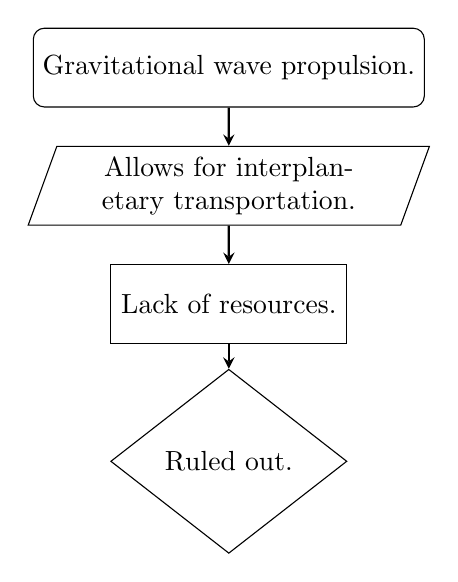
\begin{tikzpicture}
\node (start) [startstop] {Gravitational wave propulsion. };

\node (in1) [io, below of=start, yshift=-0.5cm] {Allows for interplanetary transportation.};

\node (pro1) [process, below of=in1, yshift=-0.5cm] {Lack of resources.};

\node (dec1) [decision, below of=pro1, yshift=-1cm] {Ruled out.};
\draw [arrow] (start) -- (in1);
\draw [arrow] (in1) -- (pro1);
\draw [arrow] (pro1) -- (dec1);
\end{tikzpicture}
\end{center}
\begin{center}
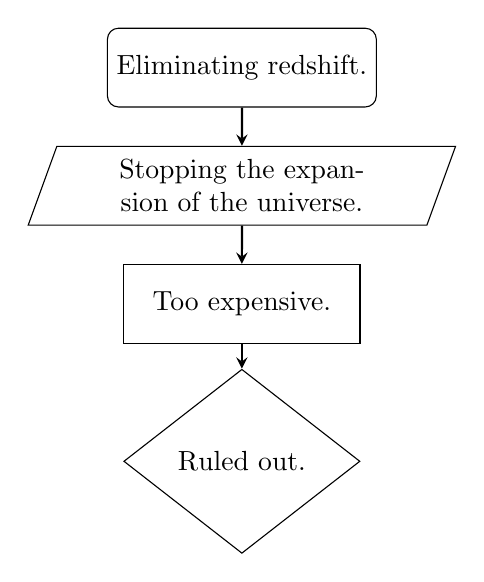
\begin{tikzpicture}
\node (start) [startstop] {Eliminating redshift. };

\node (in1) [io, below of=start, yshift=-0.5cm] {Stopping the expansion of the universe.};

\node (pro1) [process, below of=in1, yshift=-0.5cm] {Too expensive.};

\node (dec1) [decision, below of=pro1, yshift=-1cm] {Ruled out.};
\draw [arrow] (start) -- (in1);
\draw [arrow] (in1) -- (pro1);
\draw [arrow] (pro1) -- (dec1);
\end{tikzpicture}
\end{center}
\begin{center}
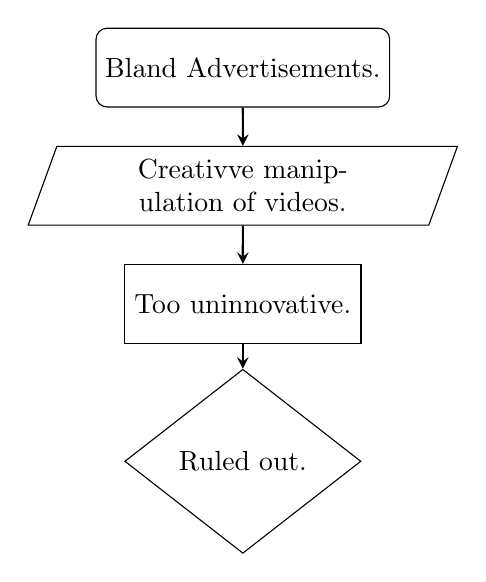
\begin{tikzpicture}
\node (start) [startstop] {Bland Advertisements. };

\node (in1) [io, below of=start, yshift=-0.5cm] {Creativve manipulation of videos.};

\node (pro1) [process, below of=in1, yshift=-0.5cm] {Too uninnovative.};

\node (dec1) [decision, below of=pro1, yshift=-1cm] {Ruled out.};
\draw [arrow] (start) -- (in1);
\draw [arrow] (in1) -- (pro1);
\draw [arrow] (pro1) -- (dec1);
\end{tikzpicture}
\end{center}
\begin{center}
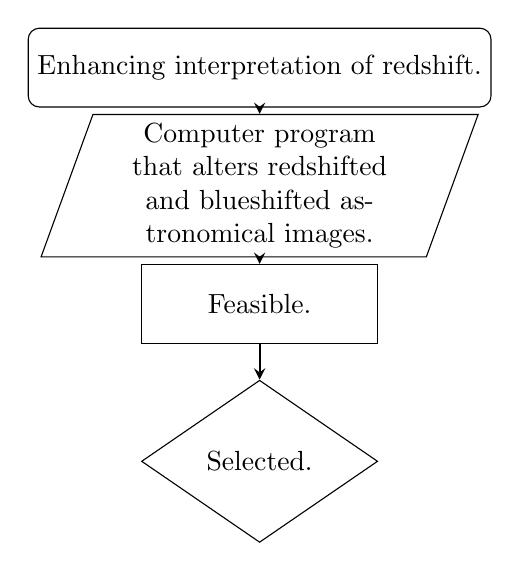
\begin{tikzpicture}
\node (start) [startstop] {Enhancing interpretation of redshift. };

\node (in1) [io, below of=start, yshift=-0.5cm] {Computer program that alters redshifted and blueshifted astronomical images.};

\node (pro1) [process, below of=in1, yshift=-0.5cm] {Feasible.};

\node (dec1) [decision, below of=pro1, yshift=-1cm] {Selected.};
\draw [arrow] (start) -- (in1);
\draw [arrow] (in1) -- (pro1);
\draw [arrow] (pro1) -- (dec1);
\end{tikzpicture}
\end{center}

\end{document}